\begin{chapter}{\label{cha:afm}Simulating the surface of a ``Floppy Wire''}
\section{Introduction}
At sufficiently low temperatures, liquid helium has two striking
properties.  Firstly, it flows without viscosity.  Secondly,
its vorticity is constrained to
thin mini-tornadoes, characterised by their fixed circulation
$h/m$ (the ratio of Planck's constant to
the mass of the relevant boson - one atom in $^4$He and one Cooper pair 
in $^3$He-B) and microscopic core radius $\xi$ 
($0.1~\rm nm$ in $^4$He and $10~\rm nm$ in $^3$He-B).  
In contrast, the eddies in everyday viscous fluids can have arbitrary shape, 
size and circulation.  

Of ongoing experimental and theoretical study is the nature of 
turbulence in superfluids 
\cite{Barenghi-PNAS,Bradley2011-NatPhys,Zmeev2015a,Boue2013}, a state 
dominated by an irregular tangle of quantised vortex lines.  Despite the fundamental differences between superfluids and classical fluids, the observations of Kolmogorov energy spectra, famed from classical isotropic turbulence, in superfluid turbulence \cite{Barenghi-PNAS} are suggestive of a deep connection between them.  Superfluid turbulence is nowadays most commonly formed by moving obstacles, including grids \cite{Davis2000}, wires \cite{Guenault1986,Bradley2005,Bradley2011,Fisher2001}, forks \cite{Blaauwgeers2007,Bradley2012}, propellers \cite{Tabeling1998,Salort2010}, spheres \cite{Schoepe1995} and other objects \cite{VinenSkrbek2008}.
Despite progress in visualizing the flow of superfluid helium in the
bulk \cite{Zmeev2015b,Duda2015}, including individual vortex reconnections
\cite{Lathrop}, there is little direct experimental evidence
about what happens at boundaries.
Here, 
vortices are believed to be generated by two mechanisms.  Firstly, 
they can nucleate at the boundary of the vessel or object.  
When the relative flow speed is sufficiently low, the flow is laminar 
{(potential)} and dissipationless.  
{Near curved boundaries, however, vortex nucleation occurs if
the local flow velocity exceeds a critical value.} 
Secondly, the vortices can be procreated from so-called `remnant vortices' 
which are present in the system since cooling the helium through the superfluid transition.  Note that remnant vortices can be avoided using judicious, slow experimental protocols \cite{Yano-2007}. 


The nano-scale vortex core in superfluid helium is comparable in size 
to the typical roughness of the boundaries of the vessel or stirring object. 
Unfortunately the lack of direct experimental information about vortex 
nucleation at the boundaries and the subsequent vortex-boundary interactions,
limit the interpretation of experiments. Theoretical
progress is challenging and to date has focussed on smooth and idealised surfaces.  In principle, the superfluid boundary conditions
are straightforward:
the superfluid velocity
component which is perpendicular to the boundary must vanish
at the boundary, whereas the tangential component (in the absence of
viscous stresses) can slip.  For the latter reason, we do not expect boundary layers,
typical of viscous flows.   
Implementing these {superfluid} boundary conditions, 
Schwarz \cite{Schwarz-1981-pinning}
and Tsubota {\it et al.} \cite{Tsubota-1994-pinning}
found that one or more vortices sliding along a smooth surface
can become deflected or trapped by a small
hemispherical bump.  Such bumps can also serve as nucleation sites for vortices;  the local superfluid velocity is raised at the pole of the bump and more readily breaks the critical velocity for vortex nucleation \cite{winiecki}.  Moreover, recent simulations \cite{Stagg-ellipse} show that, if
the bump is elliptically shaped and elongated perpendicular to the imposed flow, the superfluid velocity at the pole
is enhanced, reducing the critical velocity for vortex nucleation and increasing the vortex nucleation rate (for a given super-critical imposed flow). 
We expect therefore that microscopically-small surface roughness may promote the nucleation of vortices at a surface.
For pre-existing vortex lines in the vicinity of the surface, there is also indirect experimental evidence of a `vortex mill' mechanism 
which continuously feeds vorticity into the flow by stretching 
{the existing vortex} lines. This mechanism only works if the spooling vortex, 
held by pinning sites at the surface, is aligned in the streamwise direction \cite{Schwarz-mill}.

\begin{figure}
\centering
\includegraphics[width=0.5\linewidth]{./afm/fig1-combine-2}%
\caption{(a) AFM image of a section of the NbTi wire used to generate turbulence in superfluid helium at Lancaster University (data provided by R. P. Haley and C. Lawson).  The image has been smoothed by Gaussian blur (standard deviation 6 nm).   
(b, d, f) Magnitude of the fluid speed, $v=|{\bf v}|$, shown in the $xy$-plane and computed just above the surface (where the
density drops to $0.1 n_0$), at three times.  (c, e, {g}) Zoomed-up density isosurface plots showing the surface (yellow) and vortices (red) in the vicinity of the two tallest mountains (view taken along $y$ over the $x$-range $15 \xi \leq x \leq 125 \xi$) at the same times.  Just prior to vortex nucleation [plots (b, c), $t=20 \tau$], the largest fluid speed arises in the vicinity of the highest mountains.  When the fluid speed becomes supercritical at the highest mountains [plots (d, e), $t=30 \tau$], vortex lines becomes nucleated.  At later times [plots (f, g), $t=100 \tau$], vortices continue to be shed predominantly by the highest mountains, where the fluid speed continues to be highest.  
The nucleation vortex loops pass downstream (to the left of the mountains), filling a turbulent layer up to the height of the highest mountain.  This causes a marked downstream spreading of high fluid speed. 
}
\label{fig1}
\end{figure}
\section{Method}
To shed light on the microscopic behaviour of superflow near a rough
boundary, we work with the three-dimensional profile of a real surface, shown in Fig.~\ref{fig1}(a).  This corresponds to a one square micron region of the surface of a thin NbTi wire used to generate quantum turbulence at Lancaster University, as profiled via atomic force microscopy (AFM) \cite{Lawson}.  The surface is rough, with a height up to around 10 nm, and features sharp grooves and steep ridges, likely to have arisen during the etching phase of the wire preparation.    We assume that such a `mountain'  landscape is typical of the wires and similar objects used across other superfluid turbulence experiments.  We model the flow of
superfluid helium over this surface through the time-dependent Gross-Pitaevskii equation \cite{RobertsBerloff-GPE} (GPE) for a weakly-interacting Bose superfluid.  The superfluid is parameterised by a complex wavefunction $\Psi({\bf r},t)=\sqrt{n({\bf r},t)}\exp[i S({\bf r},t)]$, where $n$ and $S$ represent density and phase distributions, and its dynamics obey
\begin{equation}
i \hbar \frac{\partial\Psi}{\partial t} 
= \left(-\frac{\hbar^2}{2m}\nabla^2 + V({\bf r},t) + g|\Psi|^2 \right) \Psi.
\end{equation}
where $m$ denotes the particle mass, the coefficient $g$ accounts for local particle interactions, and $V({\bf r},t)$ describes a potential landscape acting on the fluid.  
The GPE is equivalent to a hydrodynamic model with fluid 
density $n({\bf r},t)=|\psi({\bf r},t)|^2$ and velocity 
${\bf v}({\bf r},t)=(\hbar/m)\nabla S$, and embodies a classical 
continuity equation and a modified Euler equation (the modification being 
the presence of a quantum pressure term, arising from zero-point motion 
of the particles {and responsible for vortex nucleation}).  
While the GPE provides only a qualitative model of the strongly-interacting superfluid helium (for example, the excitation spectrum of the GPE lacks helium's roton minimum), it nevertheless contains the key microscopic physical ingredients of our problem: finite-size vortex core, vortex interactions and vortex reconnections \cite{RobertsBerloff-GPE}.  Furthermore, any boundary, however irregular, can be conveniently
modelled through the potential $V({\bf r},t)$.  Within the GPE model and assuming a homogeneous particle density $n_0$, the vortex core size is characterised by the healing length $\xi=\hbar/\sqrt{m n_0 g}$.  The natural speed, energy and time scales are provided by the speed of sound $c=\sqrt{n_0 g/m}$, the chemical potential $\mu=n_0 g$ and the unit $\tau=\xi/c$, respectively.  

The more traditional Vortex Filament Model \cite{Schwarz1988},
which has been used to model the motion of vortex lines in the presence of
smooth spherical \cite{Hanninen-sphere,Kivotides-sphere},
hemispherical \cite{Schwarz-1981-pinning,Tsubota-1994-pinning} 
and cylindrical boundaries \cite{Hanninen-PNAS,Goto2008}, 
is less appropriate than the GPE for a number of reasons.
Firstly, it assumes that the vortex core is infinitesimal compared to 
any other length scale (which is not the case if
vortex core and wall roughness are comparable);
secondly, it does not contain vortex nucleation and kinetic energy losses due
to sound emission; thirdly it is difficult to 
generalise from smooth, geometrically simple (cylindrical or spherical)
boundaries to the rough boundaries which interest us.

Our results are based on intensive simulations of the GPE over the entire AFM surface, resolved down to a sub-core scale of $\Delta=0.4\xi$.  In $^4$He the vortex core size is $a_0 \approx 10^{-10}~\rm m$ \cite{Rayfield1964}, such that the above AFM image has true core dimensions $(10^4 \times 10^4 \times 100) a_0^3$.  It is not computationally feasible to model the corresponding range of scales directly within the GPE; as such we map the AFM image onto the largest practical healing length volume of $(400 \times 400 \times 100) \xi^3$.  This is simulated in a box of size $(400 \times 400 \times 200) \xi^3$ (the numerical domain being twice as high as the highest mountain in the third dimension), on a $1000\times 1000\times 500$ spatial grid, which is periodic in $x$ and $y$.  Time evolution is performed with 4th order Runge-Kutta scheme
with time step $\Delta t=0.01 \tau $, and performed across 256 (2.6 GHz) cores of a high-performance {computer} cluster.  The rough surface is incorporated into the GPE by setting a potential barrier $V=5\mu$ below the surface, heavily prohibiting density there; above the surface the density recovers to the bulk value $n_0$ (where $V=0$) over a lengthscale of the order of $\xi$. 

We first obtain the stationary solution of the GPE in the presence of
the rough boundary, with bulk density $n_0$.  The GPE is then transformed into a frame moving at speed $u$ in the $x$-direction (corresponding to the imposed flow) by the addition of a Galilean boost term $ i \hbar u \partial \Psi/\partial x$ to the right-hand side of the GPE.  The flow speed {is}
ramped up smoothly from zero to the final value of $u=0.6 c$; this final value is such that the critical velocity for nucleation is comfortably exceeded. 

\section{Three-dimensional results}
\begin{figure}
\centering
\raisebox{0.8cm}{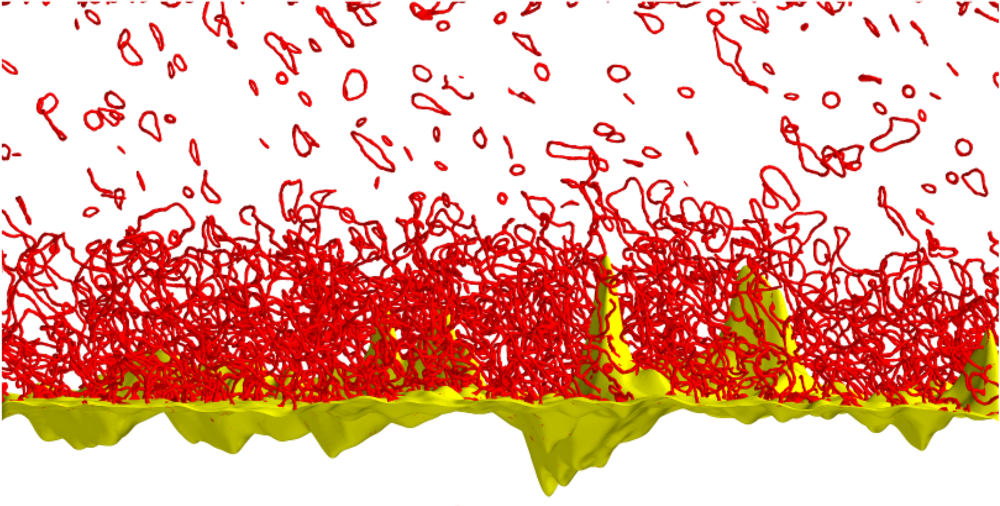
\includegraphics[width=0.5\linewidth]{./afm/fig2-2a}}%
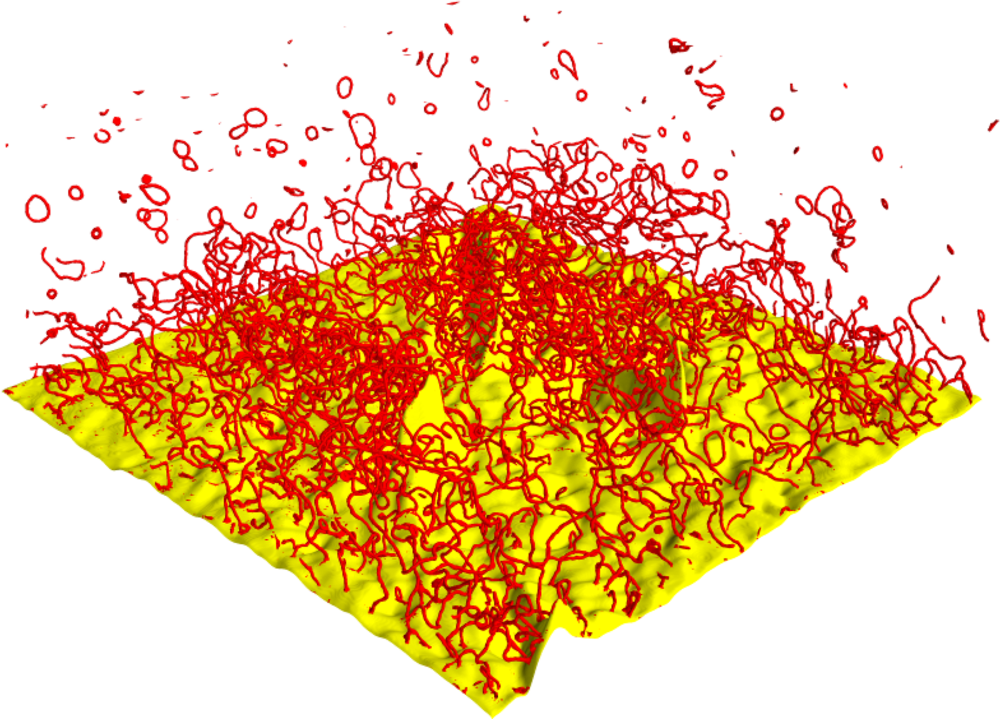
\includegraphics[width=0.5\linewidth]{./afm/fig2-2b}%
\caption{Instantaneous isosurfaces of density $n({\bf r},t)$ 
(plotted at 25\%  of the bulk density) for a super-critical flow ($u=0.6 c$) in the saturated 
turbulent regime reached at long times ($t=1220 \tau$).  Notice the turbulent boundary layer up to
approximately the height if the highest mountains and the region
of small vortex rings above it.}
\label{fig2}
\end{figure}  
{In the vicinity of the surface the local fluid speed}, $v=|{\bf v}|$, 
is enhanced considerably by the {surface's} roughness, 
with the maximum values occurring near the tallest mountain [Fig. 1 (b)].   Up to a critical imposed speed, the flow remains laminar and free of vortices.  For increased imposed flow velocity, the critical velocity is first exceeded at the highest mountain, leading to nucleation of a vortex line [Fig. 1 (e)], and then by other high mountains on the surface.  The critical velocity for vortex nucleation across this surface occurs for an imposed flow $u_c\approx 0.2 c$; this is considerably smaller than, say a hemispherical bump for which $u_c \approx 0.5 c$ \cite{winiecki},  indicating the significant role of the surface roughness in enhancing the breakdown of laminar flow.  

Nucleated vortices either peel off the boundary, or, more frequently, slide
down the slopes of the mountains (carried by the imposed flow) in the form of partially attached vortex loops.
Such loops then interact with other vortices, becoming more distorted, and forming a tangle of vortices downstream of the mountains [Fig. 1(g)].  This tangle of vortices is continuously fed by further vortices nucleated from the mountains.  The spreading of the velocity plots in Figs.~\ref{fig1} (b, c) reveals
the formation of clusters of vortices on the leeward side of the mountains, which eventually saturate a
turbulent layer.  Vortex lines occasionally undergo vortex reconnections, or twist, detach and fly off as small 
vortex rings. At later times and higher imposed flow velocities, the critical velocity is exceeded across greater areas of the surface.  However, even after considerable vortex nucleation, the highest mountains continue to dominate the vortex nucleation - here the fluid velocity is always the highest [Fig. 1(f)] and vortex shedding occurs at the fastest rate. This confirms that, with our choice of parameters,
the vortex tangle which develops can be interpreted as generated either
intrinsically or extrinsically: in both cases vortices nucleate 
at the highest mountains before filling the layer below.
Indeed, Fig.~1(g) shows the formation of a long curved
vortex which becomes twisted generating more vorticity  by spooling smaller vortex loops, 
as in the vortex-mill mechanism envisaged by Schwarz \cite{Schwarz-mill}.

As the number of vortices increases, a complex,
turbulent region consisting of superfluid vortex loops and rings is 
formed [Fig.~2 (a,b)].  This is strongly localised to the vicinity of the surface, up to approximately the height of the highest mountain. Reconnections due to twisting of vortex lines or interaction of neighbouring lines form a continuous ejection of vortex rings which spread into the bulk, visible in
the upper part of Fig.~2(a, b). The vortex length in the vicinity of the boundary, which has so far been increasing, approximately saturates in value. {A supplementary movie \cite{supp} shows the full evolution of the turbulent layer.}   For slower, but still super-critical, imposed flows the turbulent layer still forms with the same height, albeit with reduced density of vortices.

The turbulent
layer is not isotropic: on the average, vortex lines are 
flattened parallel to plane of the surface
(the areas covered by vortex cores on
the lines of sight along the $x$ and $y$ directions are only 62 and 60$\%$ 
respectively of the same area along the $z$ direction).  

%\section{\label{section:sfwire} Superfluid wire experiments}
%Developments in flow visualization at very low temperatures
%\cite{Guo2014,Fisher2014} have
%driven recent progress in the turbulence in superfluid $^4$He and
%$^3$He-B. Experiments and theory have highlighted effects
%such the existence of classical and
%nonclassical turbulent regimes \cite{WalmsleyGolov2008}, and
%energy transfer over length scales, both
%direct \cite{Barenghi2014} and inverse
%\cite{WalmsleyTompsett2013,Baggaley2014}.
%At the same time, improvements in the generation, observation and control of quantum
%vortices in atomic Bose--Einstein condensates\cite{Henn,Freilich2010,aioi11,neely_bradley_13,kwon_moon_14}
%has added a character of interdisclinarity to the study of
%turbulence in quantum fluids.

%In many superfluid helium experiments \cite{VinenSkrbek2008}, turbulence
%is generated by moving grids \cite{Davis2000},
%wires \cite{Guenault1986,brad05,Bradley2011,Fisher2001,goto08},
%forks \cite{Blaauwgeers2007,Bradley2012} or spheres \cite{Schoepe1995}.
%Although macroscopically polished, the surface of these objects is
%rough on the length scale of the superfluid vortex core, which is of
%the order of $10^{-10}~\rm m$ in $^4$He
%and $10^{-8}~\rm m$ in $^3$He.  As an example, Fig.~\ref{fig:afmimg}(a) is an atomic force microscope (AFM) image showing the microscopic detail on the surface of a  single--core NbTi `floppy' wire used for generating superfluid turbulence  \cite{Bradley2011}.  Note the appearance of an elongated scratch, typical of such wires.  No direct flow visualization is available on these microscopic length scales and, as such, 
%superflow in the presence of walls remains poorly understood. In principle, the superfluid boundary conditions should
%be straighforward.
% the simplest case of a boundary at rest, the superfluid velocity
%component which is perpendicular to the boundary must be equal to
%zero at the boundary, while the tangential component can slip.
%In practice, nucleation of quantum vorticity complicates
%this idealized Eulerian picture.

%The established theoretical approaches used to successfully describe
%homogeneous superfluid turbulence away from boundaries can falter in the presence of realistic boundaries.
%First consider the vortex filament method of Schwarz
%\cite{Schwarz,Hanninen-PNAS}. Its application to relatively simple and smooth
%boundaries, such as spheres \cite{Hanninen-sphere,Kivotides-sphere} and
%hemispheres \cite{Schwarz-bump}, has proved
%cumbersome due to the complex system of images which is required.
%Its starting assumption, that the vortex core
%is infinitesimally smaller than any other length scale, makes it
%unsuitable for realistic boundaries of roughness comparable to
%the vortex core size.  Moreover Schwarz's approach requires arbitrarily seeding
%vortex loops, because it does not account for vortex nucleation.
%Another approach which suffers similar difficulties \cite{Henderson} is
%the two--fluid Hall--Vinen--Bekarevich--Khalatnikov (HVBK)
%equations \cite{Salort2011,Salort2012}. Moreover, the HVBK equations are coarse--grained over
%length scales larger than the average vortex separation, hence the
%boundary conditions require further assumptions or the introduction of
%unknown sliding/pinning parameters.

%A practical dynamical model of superflow near boundaries of arbitrary
%shape which is powerful enough to describe vortex nucleation is
%the Gross--Pitaevskii equation (GPE) \cite{RobertsBerloff}.  While the GPE is an accurate quantitative description of atomic condensates, it provides only a qualitative model of superfluid helium.  Frisch {\it et al.} pioneered the GPE approach by simulating superflow past a cylinder, observing vortex pair nucleation above a critical flow speed \cite{frisch92}.  Subsequent GPE-based works have further elucidated vortex generation past a cylinder \cite{nore93,jma99,saito10}, as well as spheres and half-spheres \cite{winiecki99}, and elliptical objects \cite{stagg_parker_14}.    Nevertheless, at this stage of investigation, the GPE is the optimum tool 
%to gain physical insight into the flow of a superfluid over
%rough surfaces typical of experiments.

%Our numerical approach is to first obtain the stationary solution for the static fluid $(v=0)$, achieved via imaginary time propagation of the GPE \cite{Minguzzi2004}.  From this initial condition the GPE is then propagated in real time, with the fluid speed $v$ ramped up smoothly from zero up to its required value.  

\section{Two-dimensional results}
\begin{figure*}
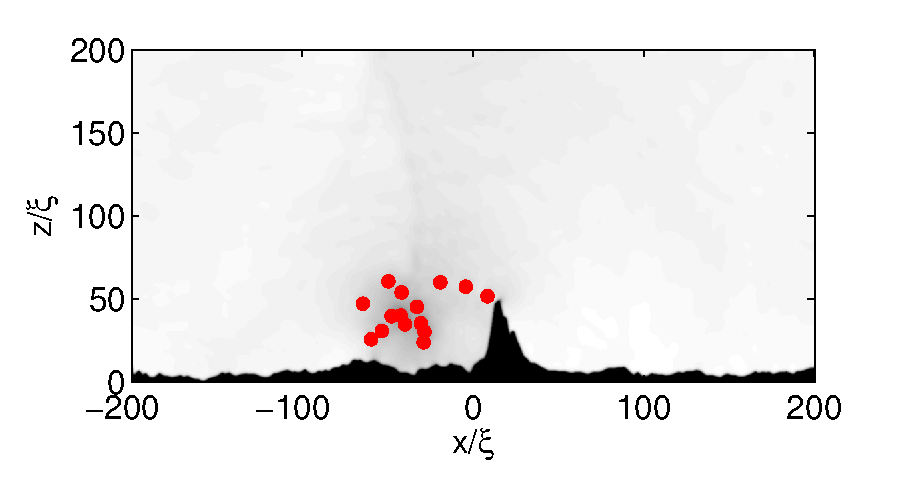
\includegraphics[width=0.35\linewidth]{./afm/figures/prog-35-500}\hspace{-0.6cm}
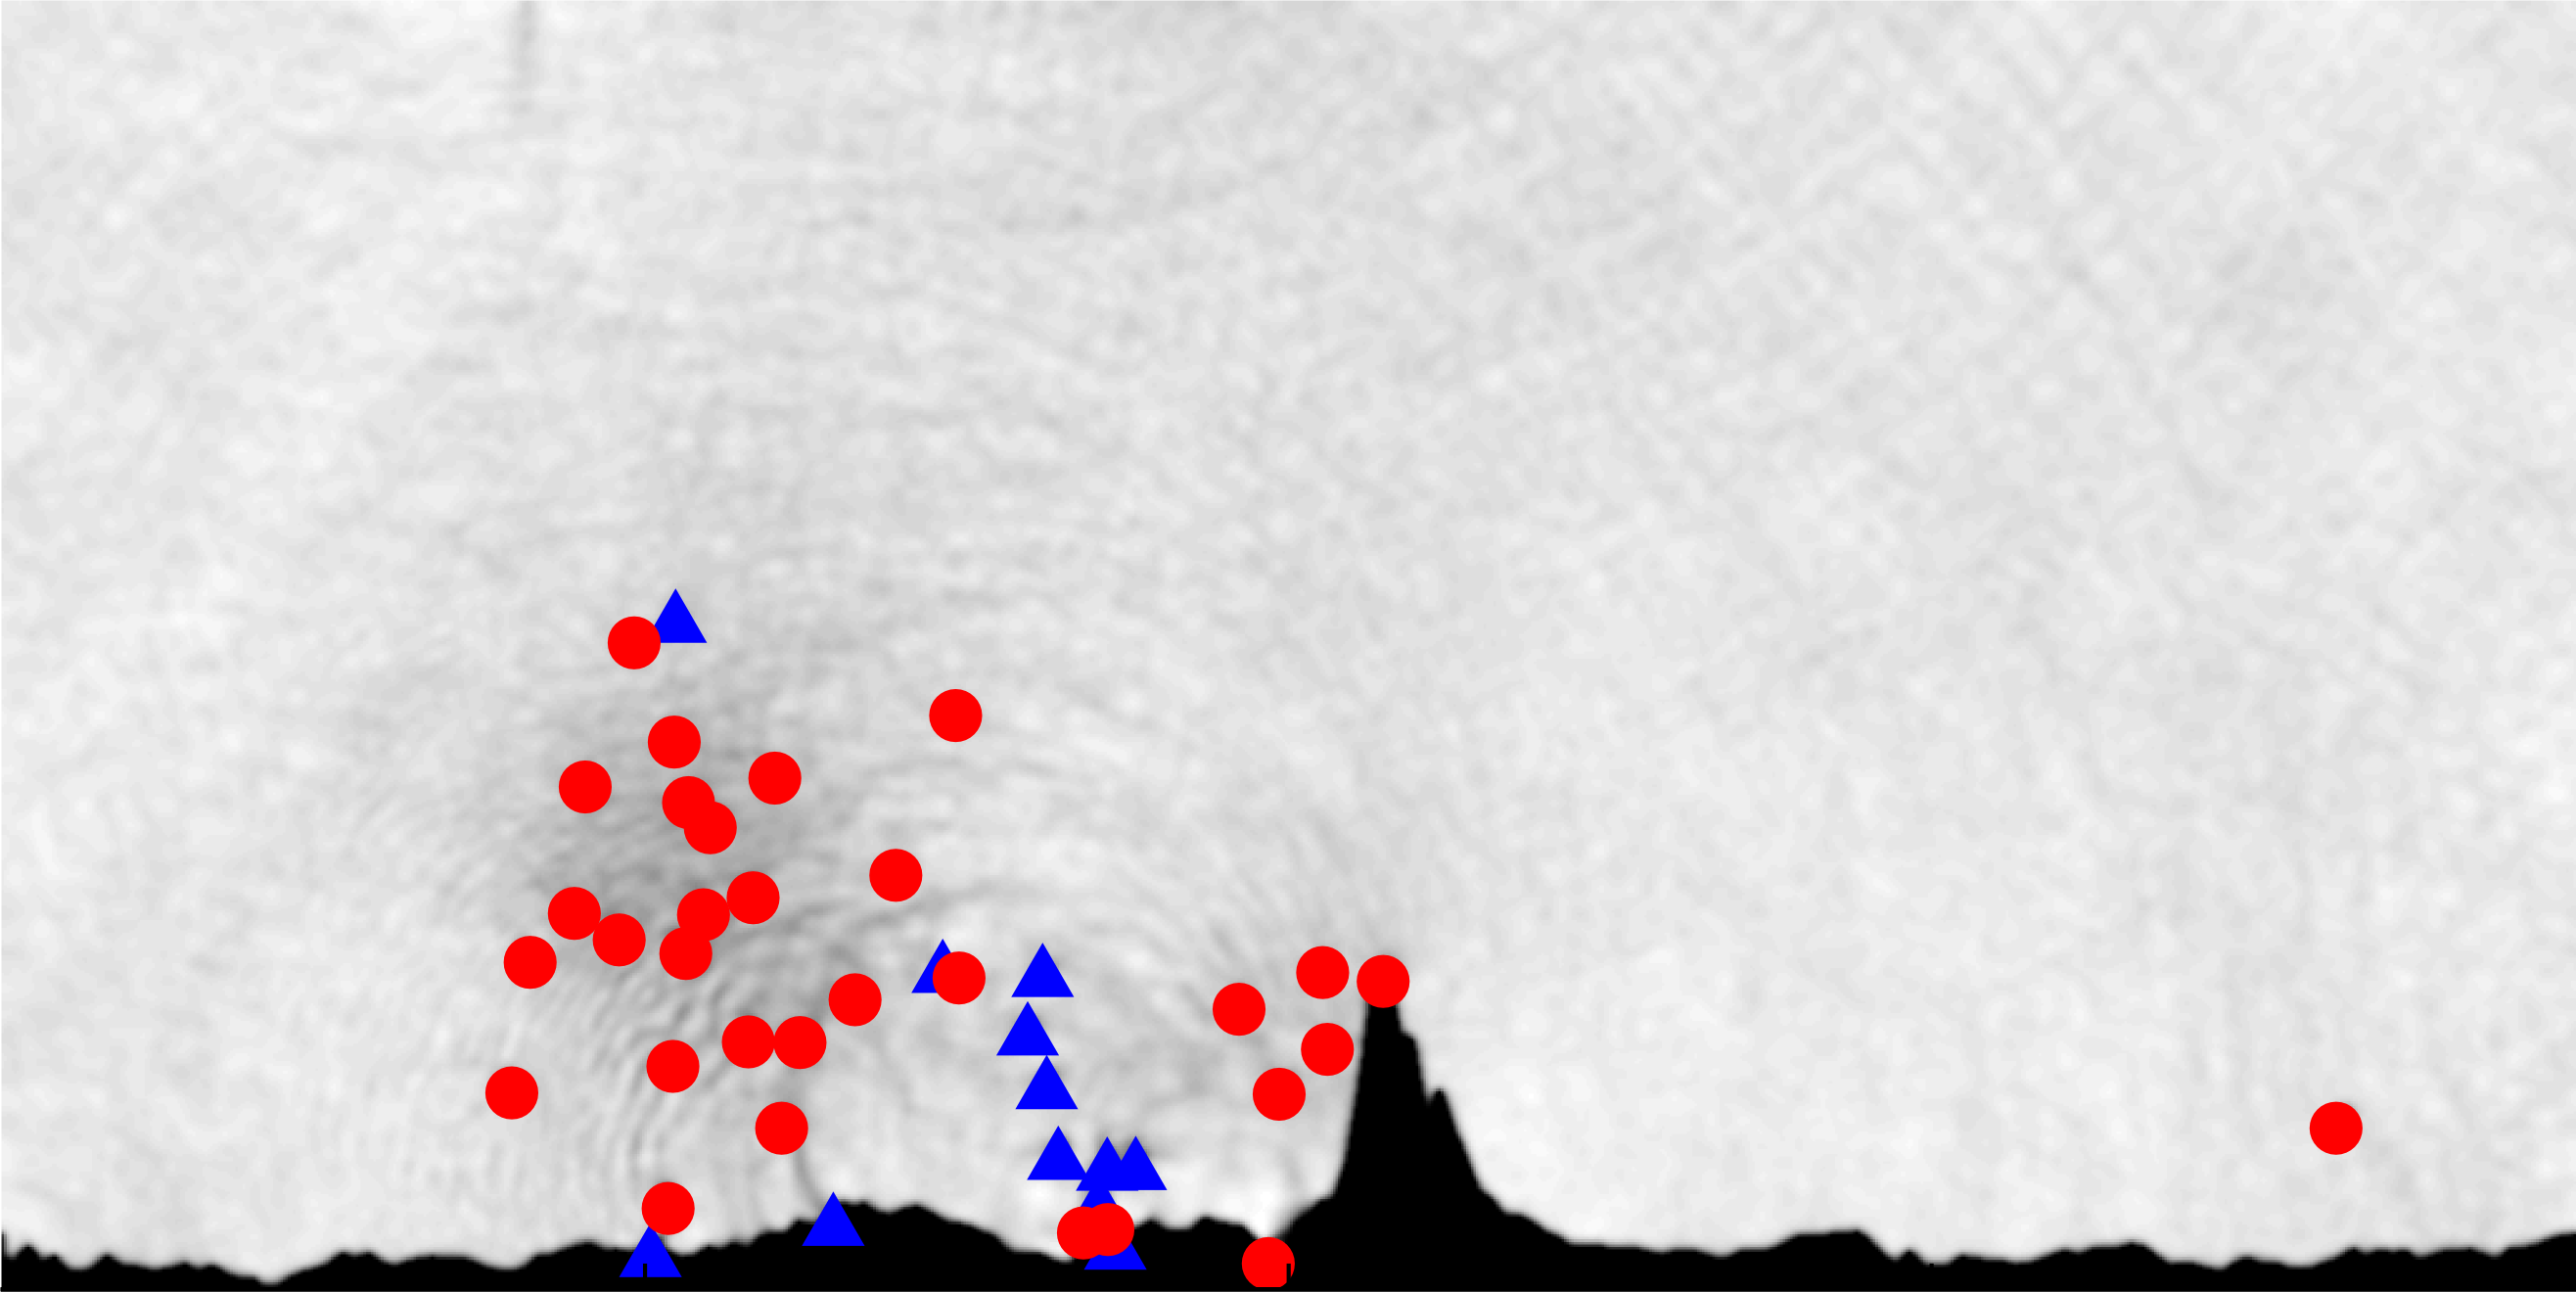
\includegraphics[width=0.35\linewidth]{./afm/figures/prog-35-1580}\hspace{-0.6cm}
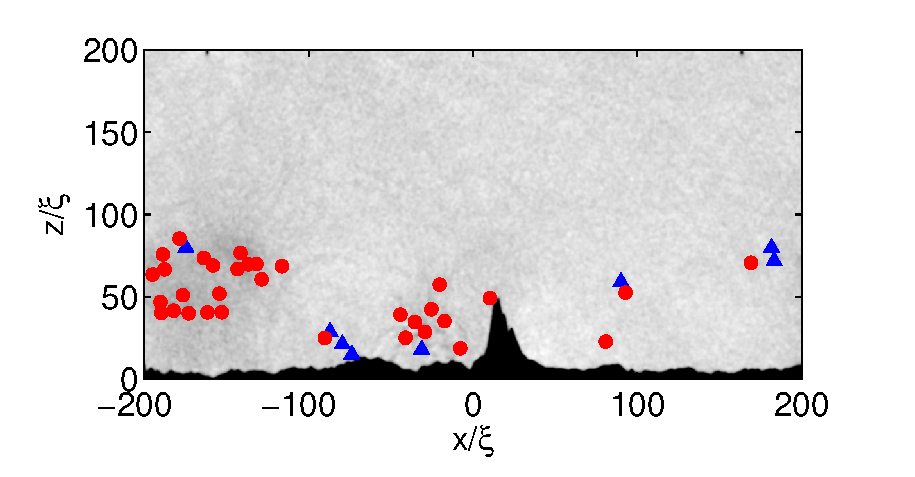
\includegraphics[width=0.35\linewidth]{./afm/figures/prog-35-2100}
\caption{\label{fig:prog} Evolution of 2D flow past the rough surface for a flow speed of $v=0.35c$.  Depicted are snapshots of density and vortex locations at times (from left to right) $t=500$, $1580$, and $2100~\tau$.  Red (blue) circles represent vortices of positive (negative) circulation.  }%Cluster forms, is interupped by secondary cluster and detaches. New cluster forms. }
\end{figure*}
\begin{figure*}
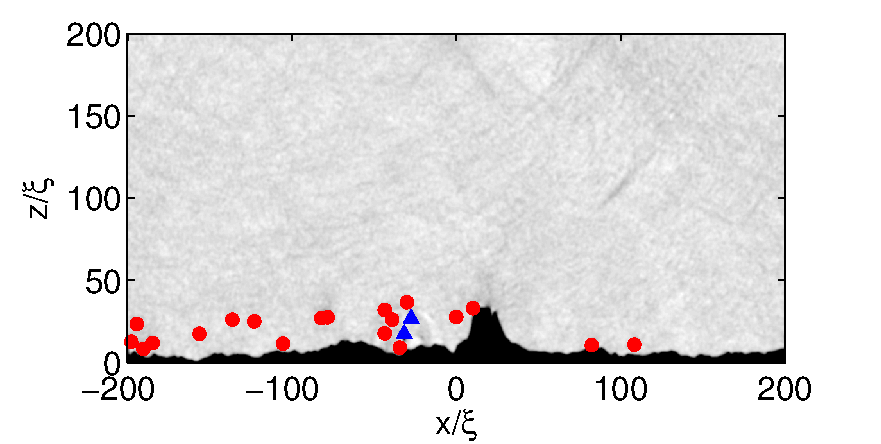
\includegraphics[width=0.35\linewidth]{./afm/figures/6th-35-2440}\hspace{-0.6cm}
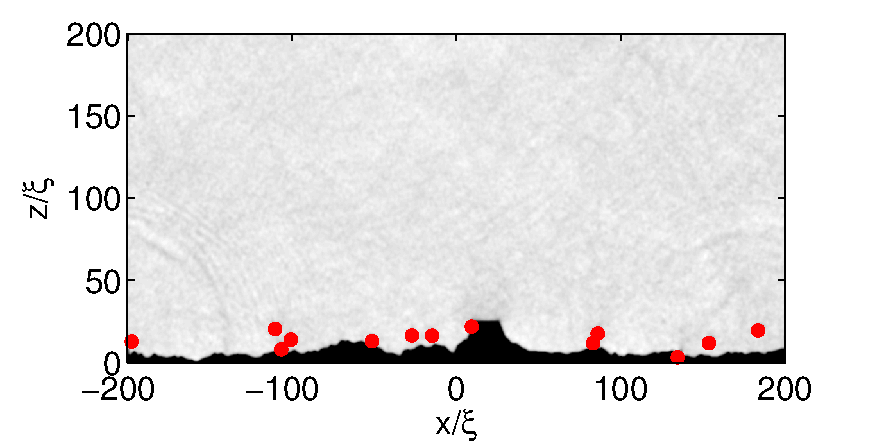
\includegraphics[width=0.35\linewidth]{./afm/figures/8th-35-2440}\hspace{-0.6cm}
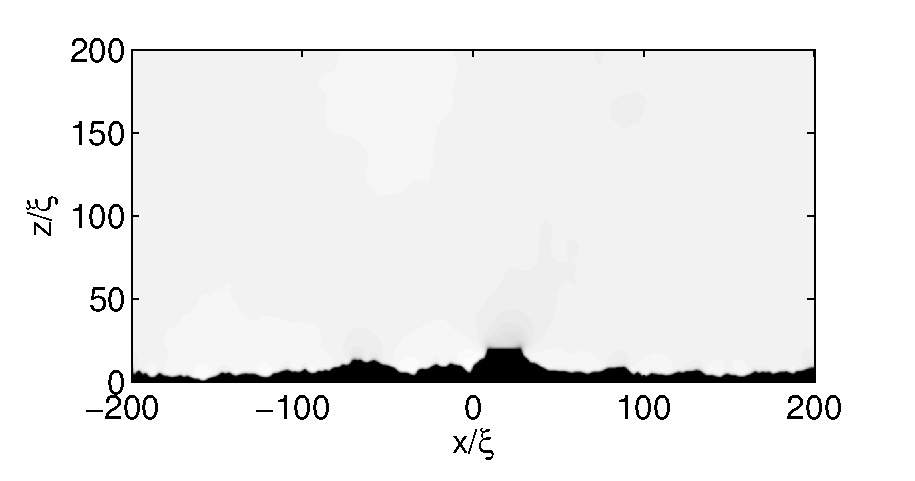
\includegraphics[width=0.35\linewidth]{./afm/figures/10th-35-2440}
\caption{\label{fig:trunc} Same-time snapshots for various levels of surface truncation: (i) $\beta=70\%$, (ii) $\beta=50\%$ and (iiii) $\beta=40\%$, where $\beta$ represents the truncation height relative to the highest point in the surface. Depicted are snapshots of density and vortex locations. For comparison, the untruncated surface ($\beta=100\%$) is depicted in Fig. \ref{fig:prog}.  The flow speed is $v=0.35c$ and the time is $t=2440\tau$.}
\end{figure*}
We find the critical velocity for vortex nucleation to be $v_c=(0.125\pm0.025) c$. We focus on an arbitrary super-critical flow speed of $v=0.35c$, with Fig. \ref{fig:prog} depicting the evolution of the system.  For clarity we show both the condensate density (upper plots) and vortex locations/circulation (lower plots).  At early times, a series of positive-circulation vortices (red) peel off from the peak of the large mountain. Vortices are nucleated here, and not elsewhere, due to the high curvature in the surface at this peak, which induces a relatively high local fluid velocity.  As they are carried downstream the vortices stay in close proximity and co-rotate about one another; this leads to the vortices combining into a larger-scale cluster of positive circulation.  This cluster travels downstream just above the surface.  Close to the surface, the cluster introduces a large relative fluid flow in the positive-$x$ direction.  This interrupts the nucleation of vortices from the mountain top and also induces the secondary generation of vortices (blue) from smaller-scale surface prominences.  These secondary vortices are of negative circulation and also form a vortex cluster. As this cluster grows, it leads to a cessation of secondary vortex production, and so again the primary vortices become nucleated from the mountain peak.  This process repeats.

The total number of vortices $N_v$ increases with time (Fig. \ref{fig:nvort}(a), solid line); initially this increase is rapid but over time it slows down as the number of vortices within the finite-sized box begins to saturate.  Initially this is almost entirely composed of positively-signed vortices (dashed line), apart from a small amount of spurious negative-sign vortices (dotted line).  At $t\approx 700 \tau$ the number of positive-sign vortices increases sharply; this represents the formation of secondary vortices. 

It is important to note that the generation of secondary clusters requires the surface to be rough downstream of the mountain.  If the surface is perfectly smooth downstream of the mountain, the positive-signed vortices persist.  

Note also that it is possible for tertiary vortices/clusters of positive-sign; these arise when the secondary cluster induces a sufficiently high flow speed in the negative-$x$ direction to generate vortices from the local surface roughness.

\subsection{Truncated surfaces}
It is evident above that the vortex generation is dominated by the large single prominence in the surface, with the smaller prominences having only a secondary effect.  To further analysis this we next study how the flow is affected by truncation of the surface height, $z=h(x,y)$, to a percentage $\beta$ of the maximum height $h_0$, i.e. $h(x,y) \rightarrow h(x,y) H(z/h_0=\beta)$, where $H(z)$ is the Heaviside step function ($\beta=100\%$ corresponds to no truncation, $\beta=0$ corresponds to complete truncation).

Figure \ref{fig:trunc} shows a snapshot (at fixed time) for various levels of truncation $\beta$, with all cases having the same flow speed $v=0.35c$.  It is evident that the height of the mountain plays a critical role.  Already, when the mountain is capped at $70\%$, the number of vortices produced by that time is vastly reduced.  The vortices are generated at a sufficiently low frequency that only small clusters form; secondary vortices are still formed but in a much lower quantity.  For $\beta=50\%$ even fewer vortices are produced, and for this case no clustering takes place and in turn no secondary vortices are formed.  For $\beta=40\%$ no vortices are generated at all.  

\begin{figure}
\centering
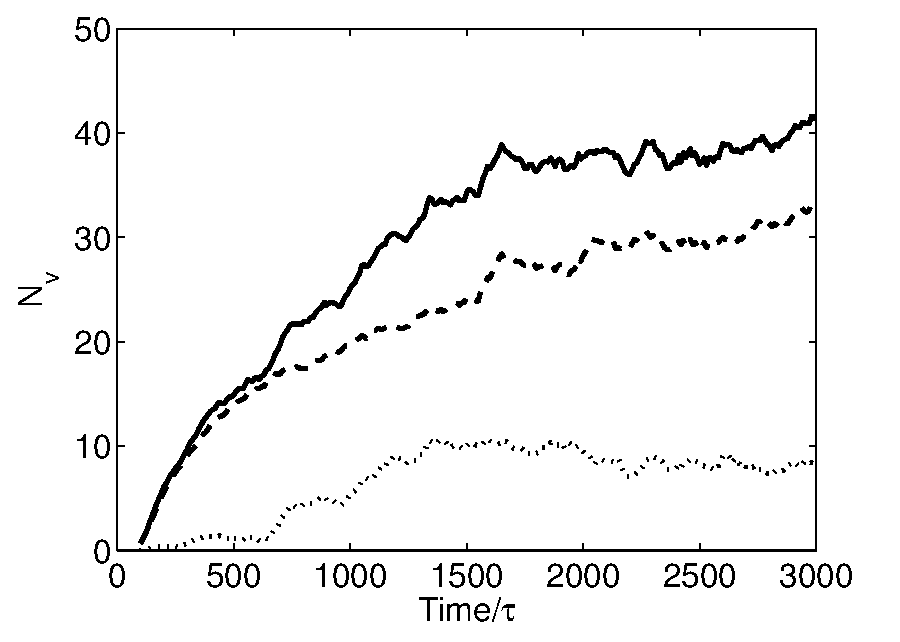
\includegraphics[width=0.45\linewidth]{./afm/figures/nvpn3bw}
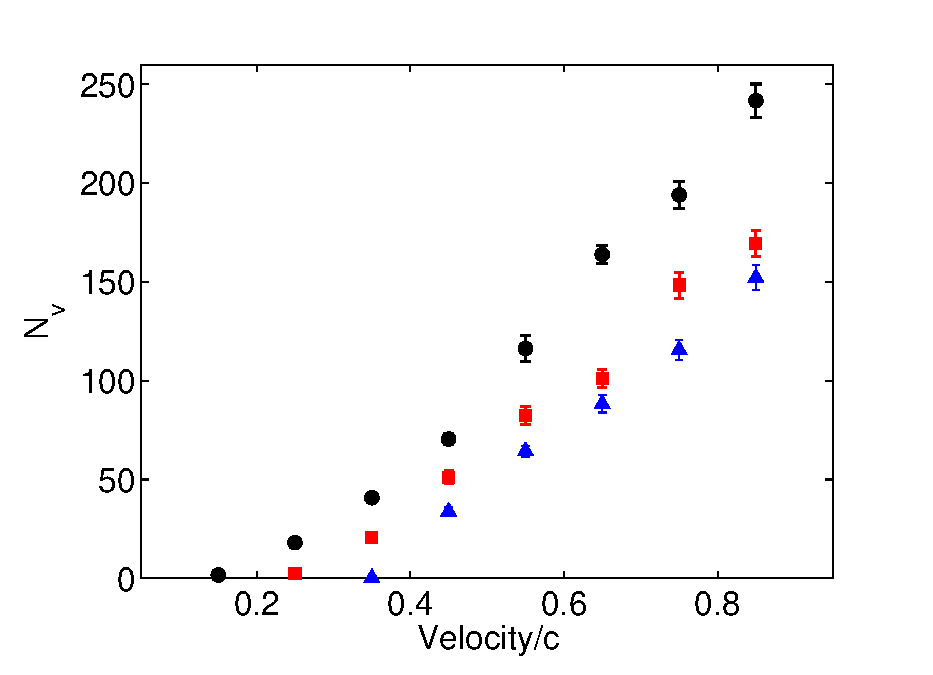
\includegraphics[width=0.45\linewidth]{./afm/figures/nv_v}
\caption{\label{fig:nvort} (a) Number of vortices produced during $v=0.35c$ flow past the surface.  Shown are the numbers of total vortices $N_v$ (solid line), positive vortices (dashed line) and negative vortices (dotted line). (b) Final number of vortices $N_v$ as a function of the flow velocity $v$ for the 2d simulations.  Each data point represents the average of 20 measurements of $N_v$ in the vicinity of $t=3000\tau$.}
\end{figure}  

\section{Conclusions}
In conclusion, our results suggest that the walls of channels which
confine the flow of superfluid liquid helium and the surfaces of moving
objects (wires, grids, propellers, spheres) which are used
to generate superfluid turbulence in current experiments
may be covered by a thin `superfluid boundary layer' consisting of 
vortex loops and rings.  This is a surprising effect, because
in fluid dynamics boundary layers usually arise from viscous forces, 
which in superfluid liquid helium near the temperature of
absolute zero are completely absent.  These findings further illustrate the deep analogies between classical and quantum fluids.
The experimental implications of `superfluid boundary layers` on macroscopic
observables need to be investigated.  Our results should
particularly stimulate experiments in $^3$He-B, where, due to relative
large healing length, it is possible to study flows with controlled 
surface height roughness. 

\end{chapter}
